\documentclass{article}
\usepackage[utf8]{inputenc}
\usepackage{amsmath}
\usepackage{bbm}
\usepackage{amsfonts}
\usepackage{aastex}
\usepackage{amssymb}
\usepackage{physics}
\usepackage{geometry}
\usepackage{fancyhdr}
\usepackage{subcaption}
\usepackage{siunitx}
\usepackage{textgreek}
\usepackage{slashed}
\usepackage{varioref}
\usepackage{hyperref}
\hypersetup{colorlinks=true, citecolor=blue, urlcolor=blue, linkcolor=black}
\usepackage{cleveref}
%\usepackage{caption}
\usepackage{tcolorbox}
\usepackage{tensor}
\usepackage[T1]{fontenc}
\usepackage{kpfonts}%  for math    
%\usepackage[scaled=0.8]{beramono}
\usepackage[scaled=0.85]{DejaVuSansMono}
\usepackage[mono=false,oldstyle]{libertine}%  serif and sans serif
\usepackage{listings}
\usepackage{xcolor}
\definecolor{codegreen}{rgb}{0,0.6,0}
\definecolor{codegray}{rgb}{0.5,0.5,0.5}
\definecolor{codepurple}{rgb}{0.58,0,0.82}
\definecolor{backcolour}{rgb}{0.95,0.95,0.92}

\lstdefinestyle{mystyle}{
    backgroundcolor=\color{backcolour},   
    commentstyle=\color{codegreen},
    keywordstyle=\color{magenta},
    numberstyle=\tiny\color{codegray},
    stringstyle=\color{codepurple},
    basicstyle=\ttfamily\footnotesize,
    breakatwhitespace=false,         
    breaklines=true,                 
    captionpos=b,                    
    keepspaces=true,                 
    numbers=left,                    
    numbersep=5pt,                  
    showspaces=false,                
    showstringspaces=false,
    showtabs=false,                  
    tabsize=2
}

\lstset{style=mystyle}
\usepackage{natbib}
\bibliographystyle{mnras}
\newcommand{\matlab}{\textsc{matlab}}
\newcommand{\tempo}{\textsc{tempo}2}
\newcommand{\libstempo}{\textsc{libstempo}}
\newcommand{\glitchhmm}{\texttt{glitch\_hmm}}
\title{Using the HMM glitch detector}
\author{Liam Dunn, Andrew Melatos, Sofia Suvorova, Bill Moran, Rob Evans}

\begin{document}
\maketitle
\tableofcontents
\section{Introduction}
This document outlines the use of \glitchhmm{}, a hidden Markov Model (HMM)-based pulsar glitch detection code which is described in detail by \citet{MelatosDunn2020}.
The purpose of \glitchhmm{} is to provide a quantitative framework for the detection of pulsar glitches based on time of arrival (ToA) data.
The package consists of three components:
\begin{itemize}
    \item A core MATLAB component which contains the HMM implementation (\texttt{matlab\_code\_logs/} in the repository).
    \item A Python library which takes a \texttt{.par} and \texttt{.tim} file and constructs an  HMM to be passed to the MATLAB code (\texttt{pulsar\_hmm/} in the repository).
    \item A Python wrapper which provides a \texttt{.ini} file-based interface to the above two components (\texttt{hmm\_wrapper/} in the repository).
\end{itemize}

The main system requirements are the following:
\begin{itemize}
    \item Python 3 
    \item A recent version of MATLAB (tested with 2018b+), with Image Processing Toolbox installed
    \item \tempo{}
    \item \libstempo{}
\end{itemize}

\section{Method overview}
This section provides an overview of the methodology and algorithms used in \glitchhmm{}. 
A comprehensive treatment is given by \citet{MelatosDunn2020}.

\subsection{Hidden Markov models in general}
\label{subsec:hmms_general}
Hidden Markov models (HMMs) provide a framework for analysing the evolution of a system whose underlying dynamics are \emph{Markovian} (memoryless) and which is observed indirectly (the true state of the system is \emph{hidden}).
The system is taken to be discrete in time, with snapshots taken at times in the set $\{t_1, t_2, \ldots, t_{N_T}\}$.
The hidden state of the system is denoted $q(t_n)$ and can take on $N_Q$ distinct values.
The evolution of the hidden state of the system is determined by a transition matrix \begin{equation} A_{q_j q_i} = \Pr[q(t_{n+1}) = q_j \mid q(t_n) = q_i]. \end{equation}
An observation of the system yields a result $o(t_n)$. 
Note that the result of an observation is not necessarily drawn from a discrete set.
The probability of an observation $o(t_n)$ given that the system is in the state $q(t_n) = q_i$ is referred to as the emission probability, and is given by \begin{equation} L_{o(t_n)q_i} = \Pr[o(t_n) \mid q(t_n) = q_i]. \end{equation}

A realisation of an HMM yields a sequence of hidden states $Q_{1:N_T} = \left\{q(t_1), q(t_2), \ldots, q(t_{N_T})\right\}$ and a sequence of observations $O_{1:N_T} = \left\{o(t_1), o(t_2), \ldots, o(t_{N_T})\right\}$.
The total probability of a particular $Q_{1:N_T}$ given the observations $O_{1:N_T}$ can be written as \begin{equation} \Pr(Q_{1:N_T} \mid O_{1:N_T}) = \Pi_{q(t_1)}L_{o(t_1)q(t_1)}\prod_{n=2}^{N_T}A_{q(t_n)q(t_{n-1})}L_{o(t_n)q(t_n)}, \end{equation}
where $\Pi_{q(t_1)}$ is the probability that the state is initalised in the state $q(t_1)$.

\subsection{Timing pulsars with hidden Markov models}
\label{subsec:hmms_timing}
To apply the HMM framework described in the Section \ref{subsec:hmms_general} to pulsar timing, we first identify the set of hidden states $\{q_i\}$ with a discrete grid of $(f, \dot{f})$ pairs which encode the instantaneous spin frequency and its first time derivative.
The grid is uniformly spaced in both directions, with $\eta_f$ and $\eta_{\dot{f}}$ denoting the space between adjacent grid points in the $f$ and $\dot{f}$ directions respectively.

We also stipulate that measurements of the system occur at each ToA measurement, and the observational datum at each timestep is the time elapsed since the last ToA measurement, i.e. $o(t_n) = t_n - t_{n-1} \equiv x_n$.
The values of $f$ and $\dot{f}$ are combined with fixed secular values $f_\text{LS}$ and $\dot{f}_\text{LS}$ measured at a reference epoch $T_0$ to give the full phase evolution \begin{equation} \Phi(t_n; f, f_\text{LS}, \dot{f}, \dot{f}_\text{LS}) = \left[f + f_\text{LS} + \dot{f}_\text{LS}(t_n-T_0)\right]x_n - \frac{1}{2}\left(\dot{f} + \dot{f}_\text{LS}\right)x_n^2. \end{equation}
The minus sign in the second term arises because we use a backwards Taylor expansion.
A secular second frequency derivative $\ddot{f}_\text{LS}$ can also be included.

The emission probability $L_{x_n q_i}$ is calculated based on the fact that the number of cycles elapsed during each ToA gap should be an integer.
This is implemented mathematically using a von Mises distribution, the precise mathematical form is given in equation 3 of \citet{DunnMelatos2022}.
The two main contributions to the variance of $\Phi(t_n; \ldots)$ are the measurement uncertainty on the ToAs, and the phase uncertainty due to the discrete gridding in $f$ and $\dot{f}$.

The evolution of the pulsar's hidden state during the gap between consecutive ToAs in the absence of a glitch is not assumed to be deterministic: we allow for some wandering in $f$ and $\dot{f}$ due to timing noise.
The default model assumes that he timing noise is driven by a white-noise torque derivative.
An explicit expression for $A_{q_j q_i}$ using this model is given by equations 10--13 and B7--B11 of \citet{MelatosDunn2020}, which also includes further discussion of this timing noise model in Section 3.4.
We also have the option to construct a model with a glitch included during a particular ToA gap.
If the model includes a glitch during a particular ToA gap, the transition matrix for that gap is modified so that the pulsar transitions with equal probability from the state $(f, \dot{f})$ to all available states $(f', \dot{f}')$ satisfying $f' > f + \dot{f}x_n$.

\subsection{Computations}
In this section we briefly describe the most common computations carried out using the HMM pulsar timing framework.
A general overview and description of common algorithms using HMMs can be found in \citet{Rabiner1989}, and further detailed descriptions of the algorithms used in this package can be found in Appendix A of \citet{MelatosDunn2020}.

Broadly speaking, there are two kinds of questions that \glitchhmm{} can be used to tackle: are there any glitches in a stretch of pulsar timing data, and what is the evolution of $f$ and $\dot{f}$ over that stretch?
These two questions are tackled through two closely related algorithms, the forward and forward-backward algorithms respectively.

\subsubsection{Glitch detection}
\label{subsec:glitch_det}
The question of glitch detection is framed as a question of Bayesian model selection.
Let $M_0$ denote the model which includes no glitches, and $M_1(k)$ denote the model which includes a glitch during the $k$th ToA gap.
For a given HMM $M$, the forward algorithm computes the model evidence $\Pr[O_{1:N_T} \mid M]$ [see Appendix A.1 of \citet{MelatosDunn2020}].
Then we can compute the Bayes factors \begin{equation} K_1(k) = \frac{\Pr[O_{1:N_T} \mid M_1(k)]}{\Pr[O_{1:N_T} \mid M_0]}. \end{equation}
Glitch candidates occur when $K_1(k)$ exceeds a predetermined threshold $K_\text{th}$, by default set at $10^{1/2}$ to achieve a false alarm rate of approximately 1\% \citep{MelatosDunn2020}.
A greedy procedure may be used to account for the possibility of multiple glitches in a stretch of data, as described in Section 4.2 of \citet{MelatosDunn2020}.

\subsubsection{Hidden state evolution}
\label{subsec:hidden_evo}
The evolution of $f$ and $\dot{f}$ is analysed through the hidden state posterior distribution $\gamma_{q_i}(t_n) = \Pr[q(t_n) = q_i \mid O_{1:N_T}]$, computed using the forward-backward algorithm [see Appendix A2 of \citet{MelatosDunn2020}].
The full posterior distribution is available as an analysis output, but it is typically more convenient to consider the posterior distributions on $f$ and $\dot{f}$ alone (marginalising over the other), denoted by $\gamma_f(t_n)$ and $\gamma_{\dot{f}}(t_n)$ respectively.
A point estimate of the evolution of $f$, $\hat{f}(t_n)$, can then be obtained by simply taking the maximum of $\gamma_f(t_n)$ at each timestep.
An analogous computation provides $\hat{\dot{f}}(t_n)$.

\section{Choosing parameters}
Putting \glitchhmm{} into practice requires the user to choose a number of parameters on a per-analysis basis.
This section describes some considerations and rules of thumb to help guide the user.

\subsection{Domain of interest}
\label{subsec:doi}
The domain of interest (DOI) refers to the set of allowed $f$ and $\dot{f}$ states in the HMM.
Recall that the hidden states specify deviations away from a secular trend (see Section \ref{subsec:hmms_timing}), so that $f = \dot{f} = 0$ indicates that the pulsar is precisely following the phase evolution specified by $f_\text{LS}$, $\dot{f}_\text{LS}$, and $T_0$.
The DOI is always set up as a uniform grid, and the boundaries and grid spacing are both important parameters.

Both the $f$ and $\dot{f}$ intervals covered by the DOI (denoted $[f_-, f_+]$ and $[\dot{f}_-, \dot{f}_+]$ respectively) must be chosen to accommodate both wandering due to timing noise and any possible glitches.
Providing a universal prescription for choosing the DOI boundaries is not feasible, but \citet{DunnMelatos2022} found that for a broad range of pulsars a frequency range of $[f_-, f_+] = [-3 \times 10^{-7}\,\mathrm{Hz}, 3 \times 10^{-7}\,\mathrm{Hz}]$ and a frequency derivative range of $[0.1\dot{f}_\text{LS}, -0.1\dot{f}_\text{LS}]$ was appropriate.

The DOI is discretised with uniform spacing in $f$ and $\dot{f}$, with spacings denoted $\eta_f$ and $\eta_{\dot{f}}$ respectively.
The choice of $\eta_{\dot{f}}$ is connected to the level of timing noise in the pulsar -- see Section \ref{subsec:tn}.
At this stage a reliable way of measuring the timing noise and turning this into a value for $\eta_{\dot{f}}$ is not at hand, and a more ad hoc method is unfortunately needed.
For example, \citet{DunnMelatos2022} chose \begin{equation} \eta_{\dot{f}} = \frac{\dot{f}_+ - \dot{f}_-}{11}, \end{equation} in combination with the prescription for $\dot{f}_{+,-}$ noted in the previous paragraph. Hence the DOI was always discretised into 11 $\dot{f}$ bins, with the bin width increasing as the magnitude of $\dot{f}_\text{LS}$ increased.
A rule of thumb for choosing $\eta_f$ depends in turn on the value of $\eta_{\dot{f}}$: it is a good idea for $\eta_f$ to be chosen so that the typical change in frequency due to a non-zero $\dot{f}$ is larger than $\eta_f$, i.e. \begin{equation} \eta_f \approx 2\eta_{\dot{f}}\langle x_n \rangle \end{equation} where $\langle x_n \rangle$ is the mean ToA gap in the dataset.
This assumes that $\eta_{\dot{f}}$ is the smallest possible non-zero value of $\dot{f}$ in the DOI, which will typically be the case.
\subsection{Timing noise}
\label{subsec:tn}
By default, \glitchhmm{} assumes that timing noise in the pulsar is driven by a white noise term in the second frequency derivative, viz. \begin{equation} \frac{\dd^2f}{\dd t^2} = \xi(t),\quad \langle\xi(t)\xi(t')\rangle = \sigma^2\delta(t-t').\label{eqn:tn}\end{equation}
This model is not intended to be a universal choice, but it has been tested on both synthetic data which includes timing noise of a manifestly different form (white noise term in frequency derivative, see \citealt{MelatosDunn2020}) and real data sets from a variety of pulsars \citep{Lower2021, DunnMelatos2022} (though note in the former reference it was found that modifying the timing noise model to include white noise in the frequency derivative instead was appropriate for a few pulsars).

The magnitude of the timing noise included in the HMM is controlled by the $\sigma$ parameter in (\ref{eqn:tn}), which has units of $\mathrm{Hz}\,\mathrm{s}^{-3/2}$.
By default, its value depends on the value of $\eta_{\dot{f}}$ (see \ref{subsec:doi}) as \begin{equation} \sigma = \eta_{\dot{f}}\langle x_n\rangle^{-1/2}\end{equation} where $\langle x_n\rangle$ is the mean ToA gap in the dataset.
The rationale behind this choice is described in 6.1 of \citet{MelatosDunn2020}.
This value can be overridden if desired -- see Listing \ref{lst:eg_ini}.


\section{Using \texttt{hmm\_wrapper}}
\label{sec:hmm_wrapper}
For the most part, analyses should be run through the scripts in \texttt{hmm\_wrapper/}, principally \texttt{run\_hmm.py}.
These scripts depend on the \texttt{pulsar\_hmm} package included in this repository --- you can install that package by running \texttt{pip install .} inside the \texttt{pulsar\_hmm/} folder.

\texttt{run\_hmm.py} takes three command-line inputs: \texttt{-\/-par}, which specifies the \texttt{.par} file to be used, \texttt{-\/-tim}, which specifies the \texttt{.tim} file to be used, and \texttt{-\/-ini}, which specifies the \texttt{.ini} file to be used.
The \texttt{.par} and \texttt{.tim} files should be \tempo{}-style files.
An example \texttt{.ini} file is shown in Listing \ref{lst:eg_ini} below.
\begin{lstlisting}[caption=Example \texttt{.ini} file, label={lst:eg_ini}]
# This section specifies the "domain of interest" (DOI), the allowed range of frequency and frequency
# derivative, and the spacing between grid points for each.
[doi]
# Minimum allowed frequency in Hz
freq_min = -3e-7  
# Maximum allowed frequency in Hz
freq_max = 3e-6 
# Spacing between frequency grid points in Hz
dfreq = 1e-8  
# Minimum allowed frequency derivative in  Hz/s
fdot_min = -1e-15 
# Maximum allowed frequency derivative in  Hz/s
fdot_max = 1e-15 
# Spacing between frequency derivative grid points in Hz/s
dfdot = 1e-16

# This section contains any parameters related to the inclusion of timing noise in the HMM
[tn]          
# Override default value of sigma specified in equation 8 (commented out for the purposes of the demo)
#sigma = 1e-20 

# This section specifies any restrictions on the ToAs to be used
[toas]
# ToAs before mjd_min will not be used
mjd_min = 58514 
# ToAs after mjd_max will not be used
mjd_max = 58700
# ToAs separated by less than min_toa_gap days will be discarded
min_toa_gap = 1                                                                        

# This section specifies where to find the relevant MATLAB code. Paths must be absolute.
[matlab]                                                       
# The path to the core MATLAB implementation (matlab_code_logs/ in the repository)
matlab_path = /fred/oz022/ldunn_glitch/glitch_hmm/matlab_code_logs_stable
# The path to the appropriate MATLAB wrapper script (usually hmm_wrapper/do_matlab_analysis.m)
matlab_wrapper = /fred/oz022/ldunn_glitch/glitch_hmm/hmm_wrapper/do_matlab_analysis.m 

# This section specifies the location of the analysis output. Paths must be absolute.
[out]
# All output files will begin with this prefix
out_prefix = /fred/oz022/ldunn_glitch/glitch_hmm/hmm_wrapper/demo/results/J1452-6036_
\end{lstlisting}

There is an example analysis waiting to be run in \texttt{hmm\_wrapper/demo/}. It uses data from {PSR J${1452-6036}$} released by the UTMOST collaboration in their first public data release \citep{LowerBailes2020}, the entirety of which can be found \href{https://github.com/Molonglo/TimingDataRelease1}{here}.
To run this demo, first edit \texttt{demo.ini} in that directory so that the variables \texttt{matlab\_path}, \texttt{matlab\_wrapper}, \texttt{working\_prefix}, and \texttt{out\_prefix} are appropriately set (noting that all paths must be absolute, not relative).
Also, make sure the directories referred to in \texttt{working\_prefix} and \texttt{out\_prefix} exist.
Then, from the \texttt{hmm\_wrapper/demo/} directory, run the analysis:
\begin{lstlisting}
$ python ../run_hmm.py --par J1452-6036.par --tim J1452-6036.tim --ini demo.ini
\end{lstlisting}
After a few minutes, several files will appear in the directory specified by \texttt{out\_prefix}.
The next section discusses these analysis results in detail.
\section{Output}
The analysis run by \texttt{run\_hmm.py} (see Section \ref{sec:hmm_wrapper}) produces quite a few output files.
In the following, we will refer to output files by their name \emph{excluding} \texttt{out\_prefix}.

\subsection{\texttt{res.dat}}
This file contains the essential details of any glitch candidates which were found in the analysis.
Each row corresponds to a glitch candidate, in descending order of significance.
The first column gives the index of the ToA gap containing the glitch candidate, and the second column gives the (natural) log Bayes factor of the glitch candidate.

\subsection{\texttt{\{f, fdot\}\_path.dat}}
These files contain  the maximum \emph{a posteriori} values of $f$ and $\dot{f}$ during each ToA gap, calculated using the model which includes all glitch candidates above the threshold.
Plots of these paths are also produced as \texttt{\{f, fdot\}\_path.pdf}.

\subsection{\texttt{\{f, fdot\}\_posterior.dat}}
These files contain the natural logarithms of the marginalised $f$ and $\dot{f}$ posteriors during each ToA gap.
Each row corresponds to a frequency (derivative) bin, in ascending order.
Plots of these posteriors are also produced as \texttt{\{f, fdot\}\_posterior.pdf}.

\subsection{\texttt{bfs.dat}}
This file contains the log Bayes factors computed in the course of the model selection procedure described in Section 4 of \citet{MelatosDunn2020}.
The procedure is a greedy one, so each iteration corresponds to calculation of new Bayes factors comparing models with all of the glitches of the most-preferred model from the previous iteration, plus one new glitch.
Plots showing the Bayes factors at each iteration are also produced, named \texttt{bfs\_i.pdf} where \texttt{i} is the iteration.

\subsection{\texttt{analysis.mat}}
Thie file contains a MATLAB workspace with the results of the analysis. 
This workspace contains all of the above data products, plus a few others which are not dumped by default.
The following is a list of important variables found in that workspace, along with a brief description:
\begin{itemize}
    \item \texttt{max\_BFs} --- contains the maximum log Bayes factors obtained in each iteration of the greedy glitch detection algorithm.
    \item \texttt{all\_BFs} -- contains all log Bayes factors calculated in each iteration of the greedy glitch detection algorithm.
    \item \texttt{fdots} --- contains the frequency derivatives in the domain of interest (DOI).
    \item \texttt{freqs} --- contains the frequencies in the DOI.
    \item \texttt{full\_posterior} --- contains the unmarginalised posterior on frequency and frequency derivative for the model selected by the glitch detection procedure.
    \item \texttt{fdot\_posterior} --- contains \texttt{full\_posterior} after marginalistaion over frequency.
    \item \texttt{freq\_posterior} --- contains \texttt{full\_posterior} after marginalistaion over frequency derivative.
    \item \texttt{glitches} --- contains the indexes of the ToA gaps during which a glitch was detected.
    \item \texttt{kappa\_per\_toa} --- contains $\kappa$ for each ToA gap, defined as the reciprocal of the squared phase uncertainty across each ToA gap (measured in radians).
    \item \texttt{path} --- contains the maximum \emph{a posteriori} path in frequency derivative (first column) and frequency (second column), calculated using the model returned from the glitch detection algorithm.
    \item \texttt{residuals} --- contains the phase residuals of \texttt{path}, measured in cycles.
\end{itemize}

\subsection{Plots}
In addition to the ASCII and \texttt{.mat} files described in the rest of this section, \glitchhmm{} also generates a number of plots in \texttt{.pdf} format.
In this subsection we describe those plots and show example plots generated from the PSR J1452$-$6036 analysis in \texttt{hmm\_wrapper/demo/}.
We emphasise that these plots are generated for convenience, and are not necessarily intended to be publication-quality -- all the data from which they are derived are available in the files described in the rest of this section.

\subsubsection{\texttt{bfs\_i.pdf}}
These plots show the log Bayes factors generated by successive iterations of the greedy model selection procedure used to detect glitches (see Section \ref{subsec:glitch_det}).
\texttt{bfs\_0.pdf} shows the first iteration, \texttt{bfs\_1.pdf} the second, and so on.
The plots generated for the PSR J1452$-$6036 example analysis are shown in Fig. \ref{fig:eg_bfs}.
\begin{figure}
    \centering
    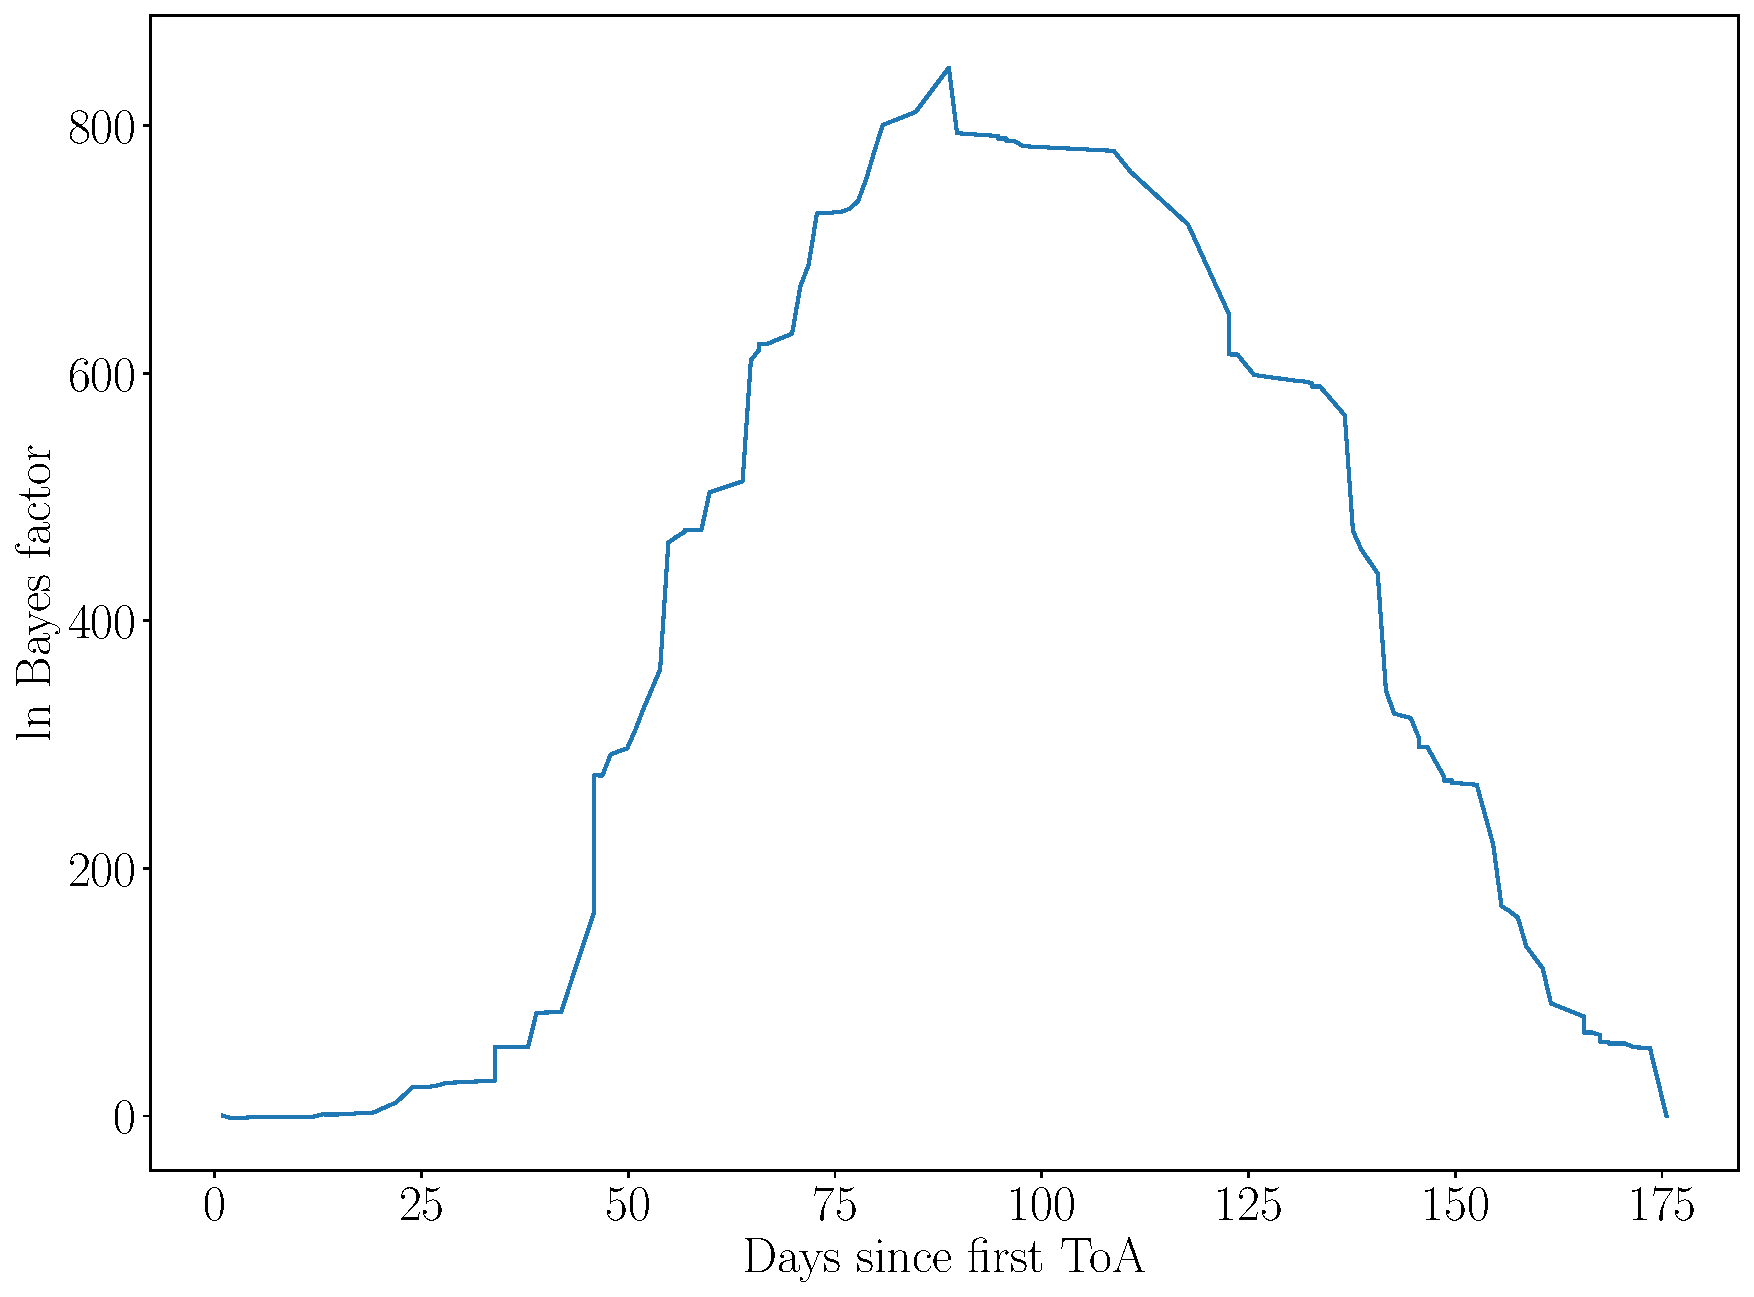
\includegraphics[width=0.5\textwidth]{figures/J1452-6036_bfs_0.pdf}
    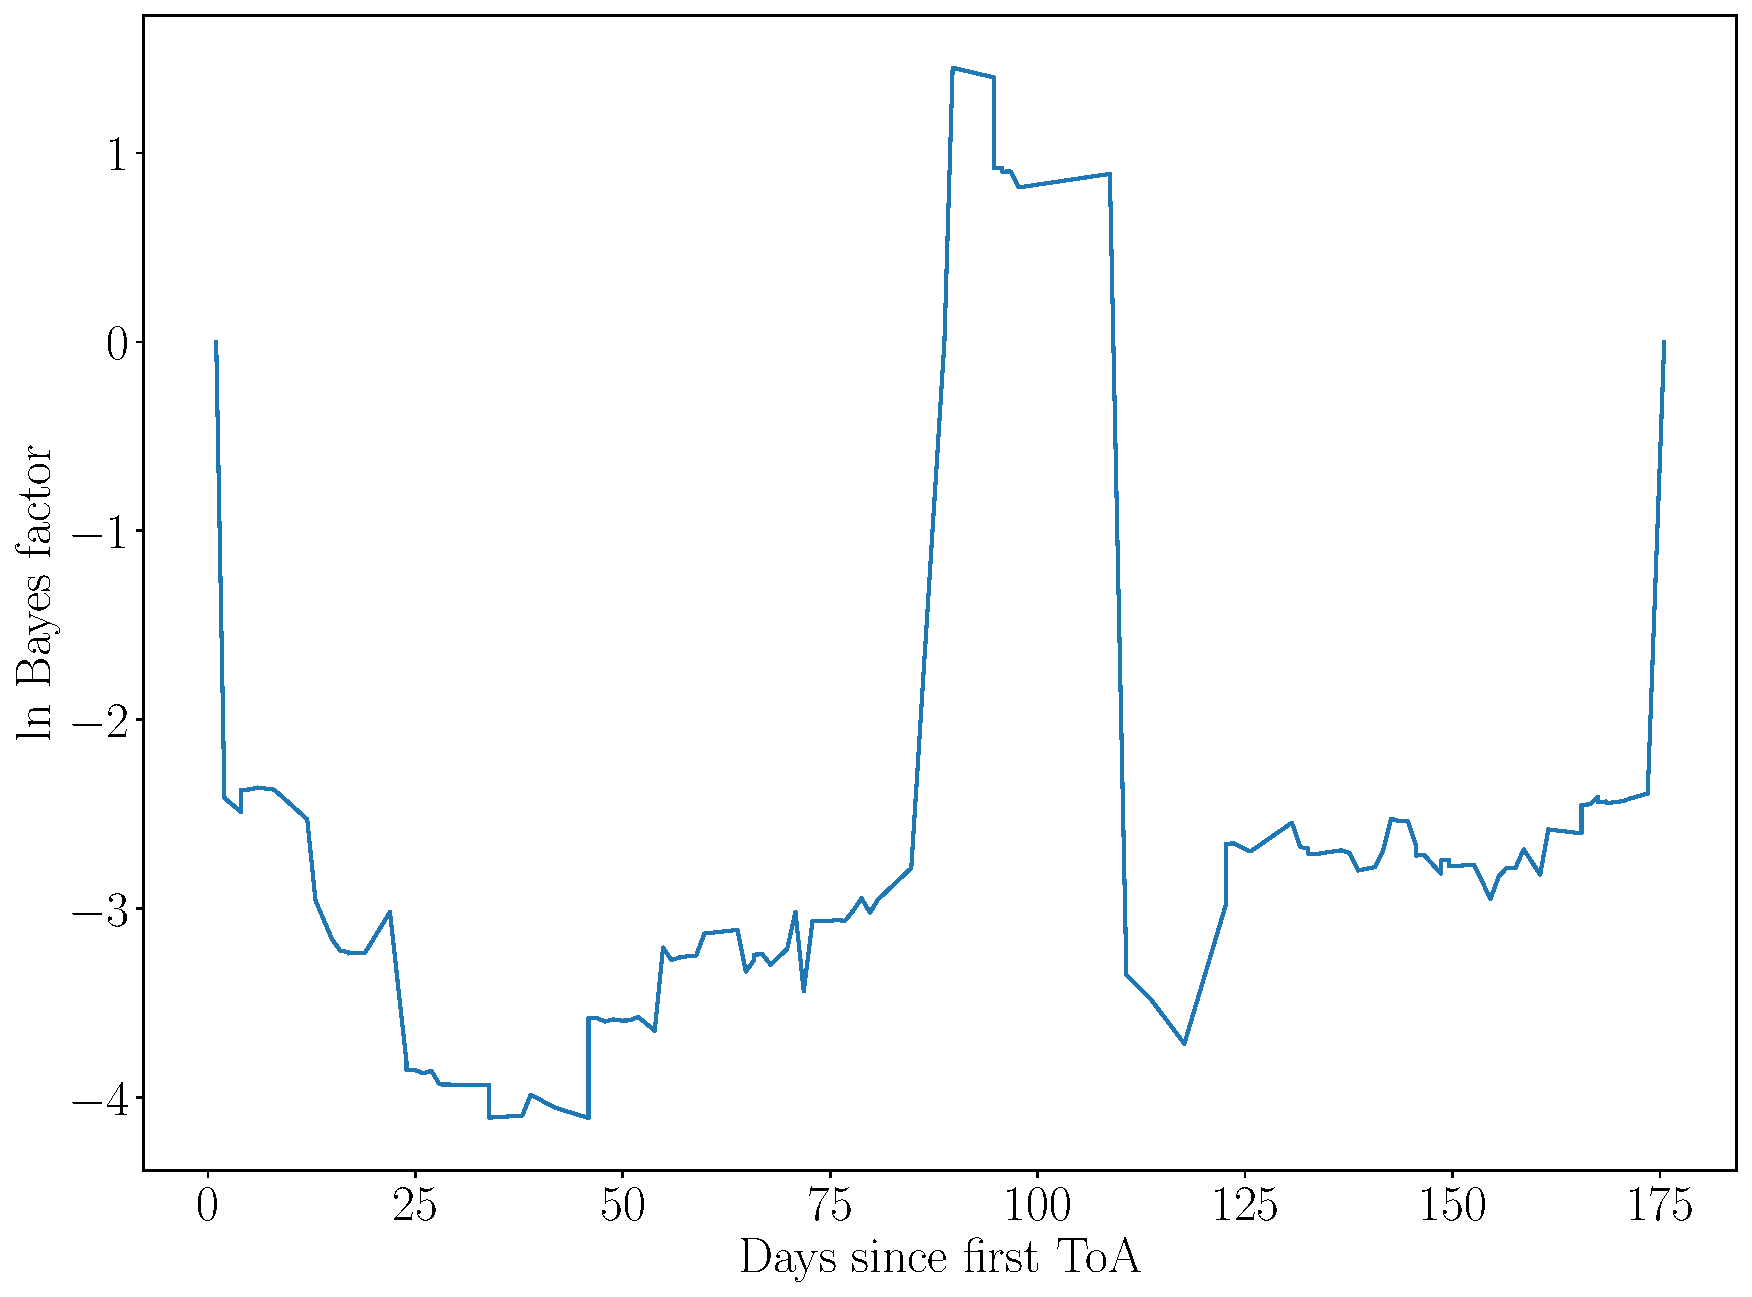
\includegraphics[width=0.5\textwidth]{figures/J1452-6036_bfs_1.pdf}
    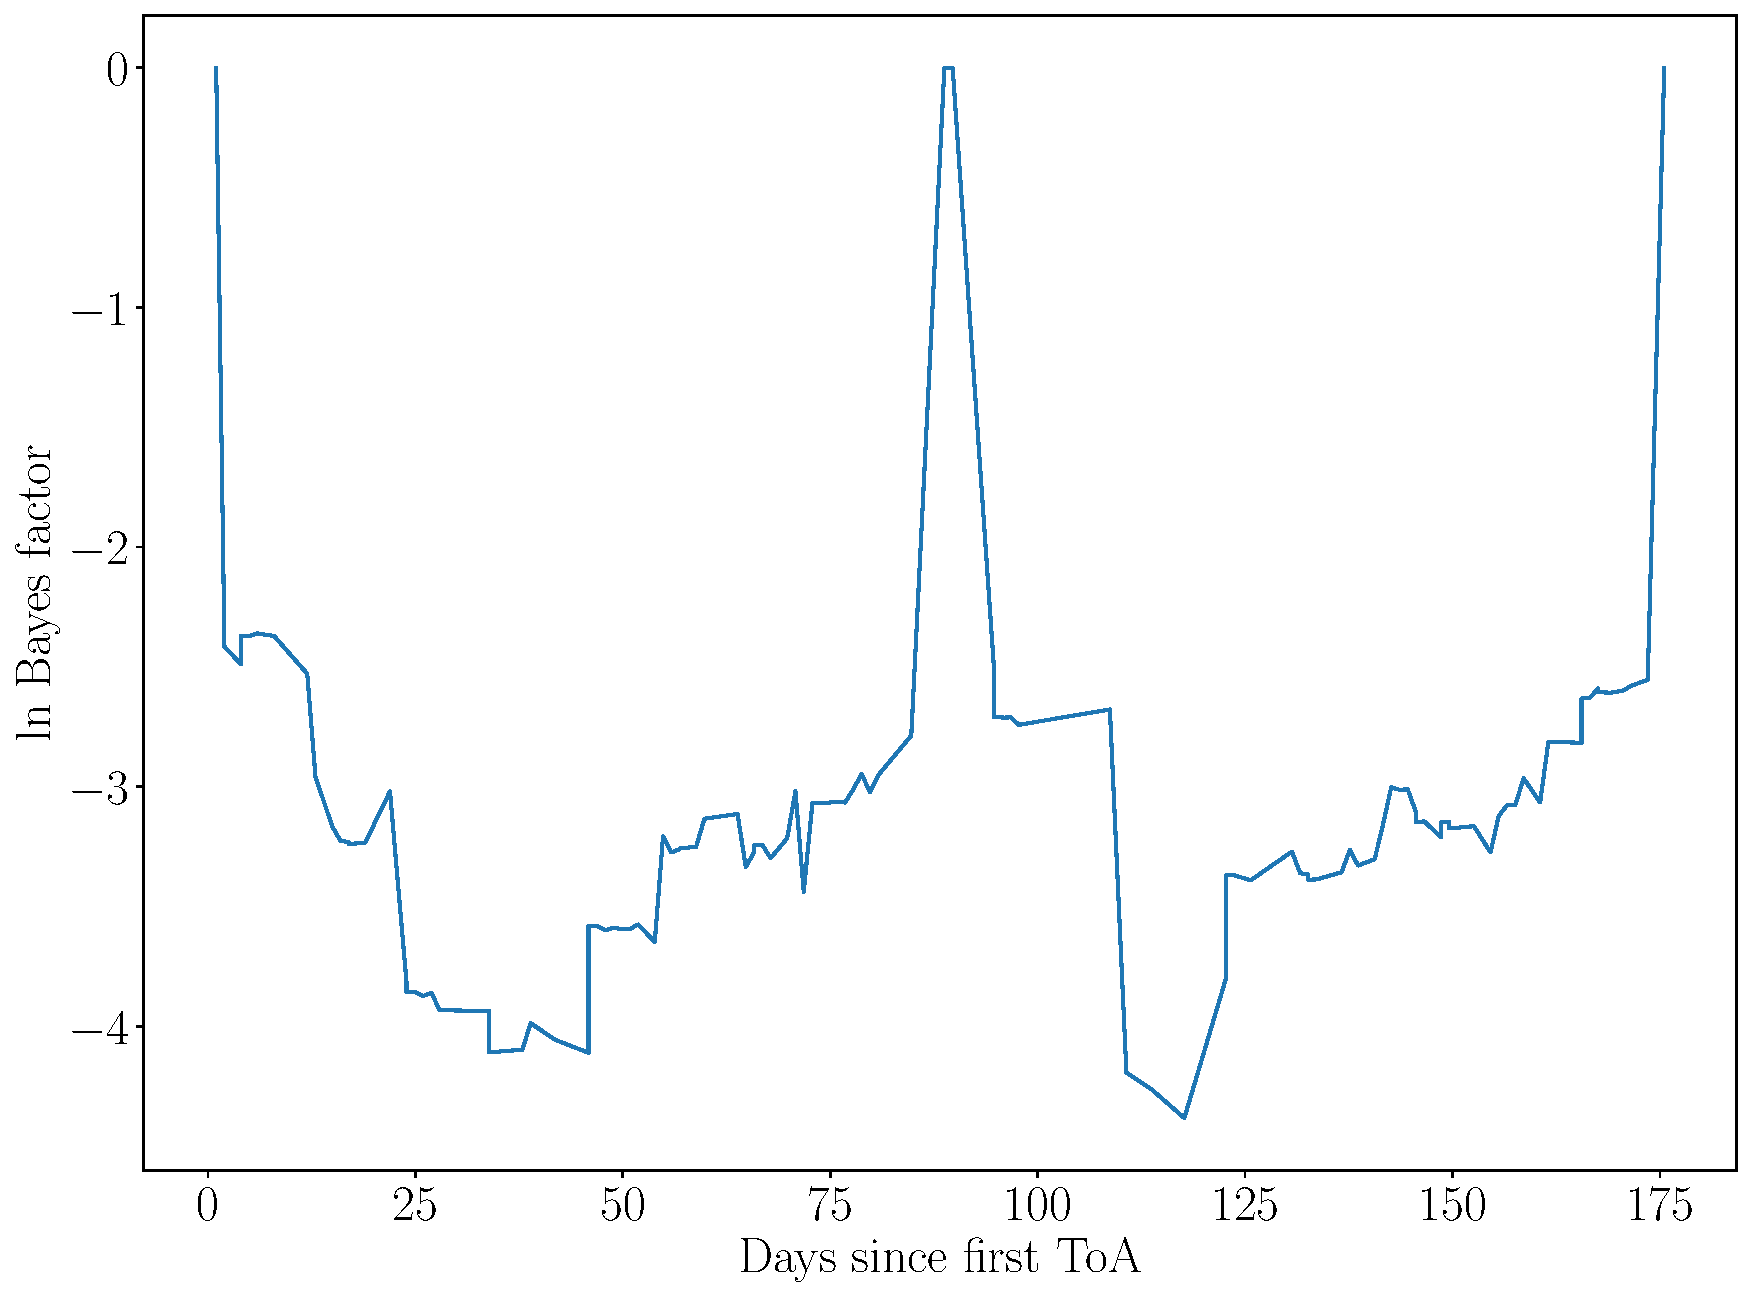
\includegraphics[width=0.5\textwidth]{figures/J1452-6036_bfs_2.pdf}
    \caption{Example \texttt{bfs\_i.pdf} plots from the demo PSR J1452$-$6036 analysis. \texttt{bfs\_0.pdf} is shown in the top panel, \texttt{bfs\_1.pdf} in the middle, and \texttt{bfs\_2.pdf} (the terminating step) in the bottom panel.}
    \label{fig:eg_bfs}
\end{figure}

\subsubsection{\texttt{\{f, fdot\}\_path.pdf}}
These plots show the sequence of most likely hidden $f$ and $\dot{f}$ states at each timestep (see Section \ref{subsec:hidden_evo}).
The plots generated for the PSR J1452$-$6036 example analysis are shown in Fig. \ref{fig:eg_paths}.
\begin{figure}
    \centering
    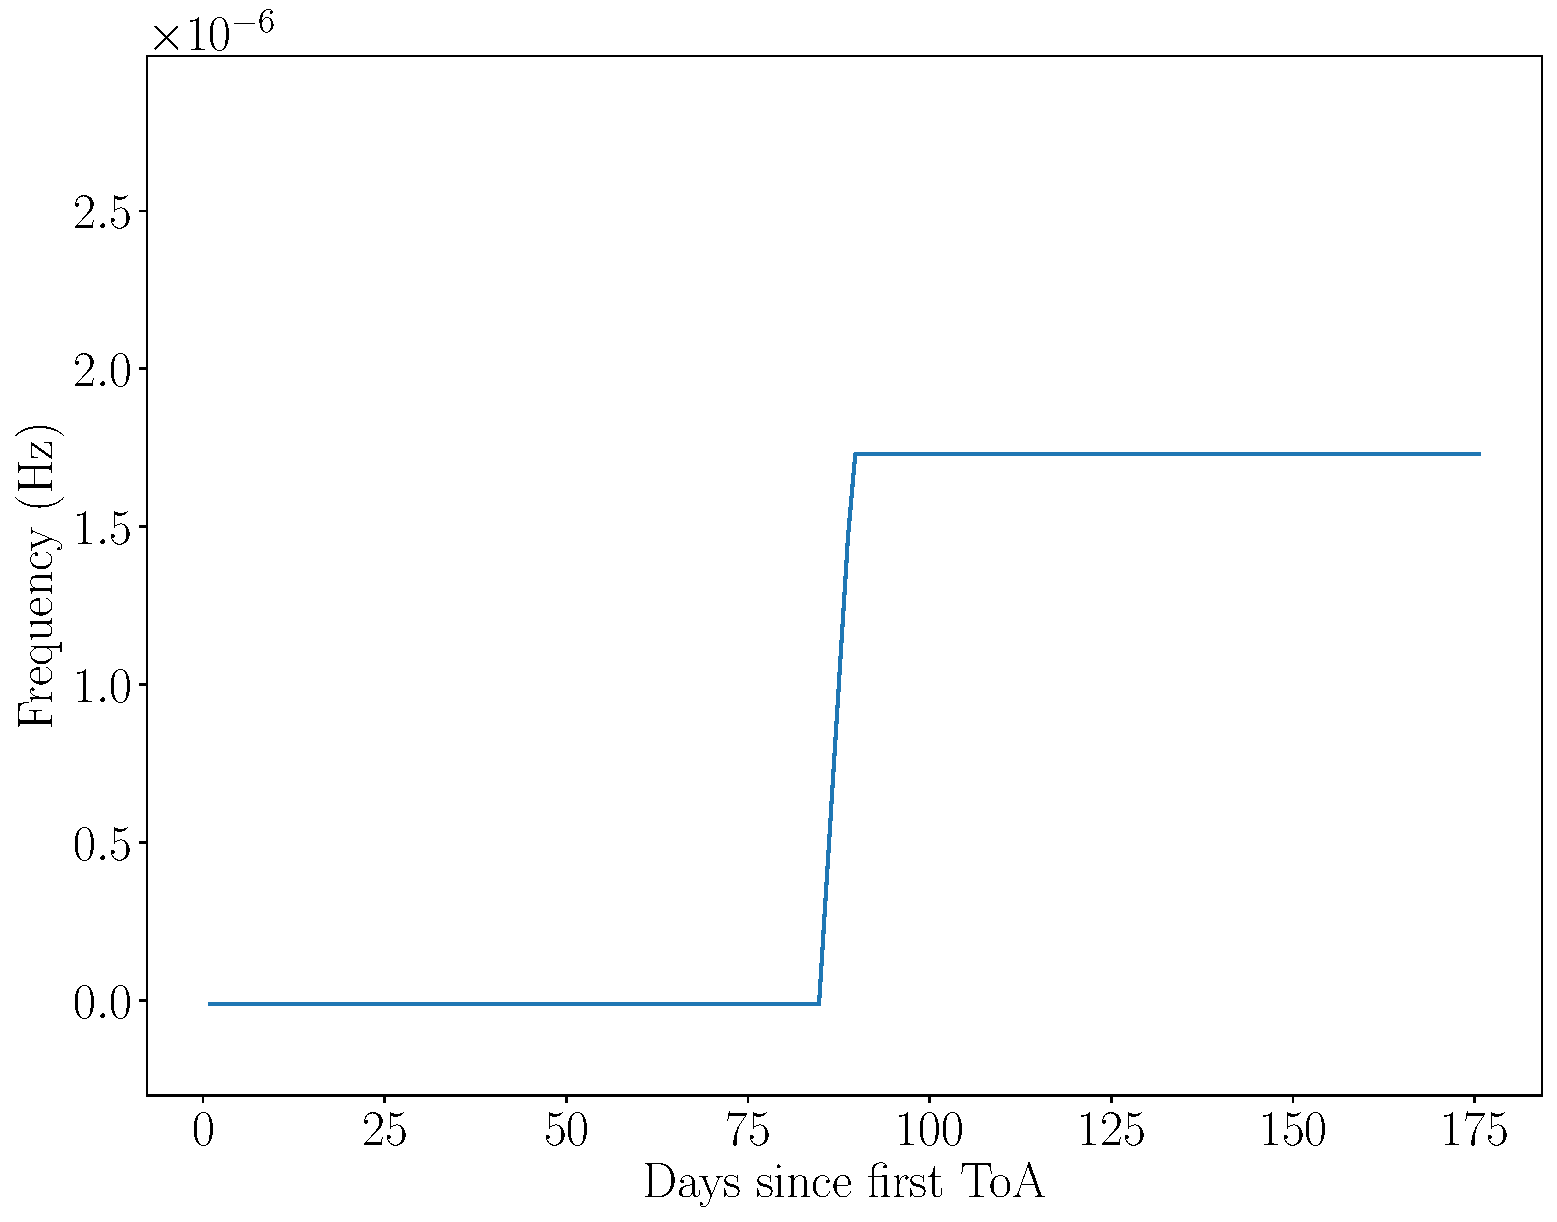
\includegraphics[width=0.49\textwidth]{figures/J1452-6036_f_path.pdf}
    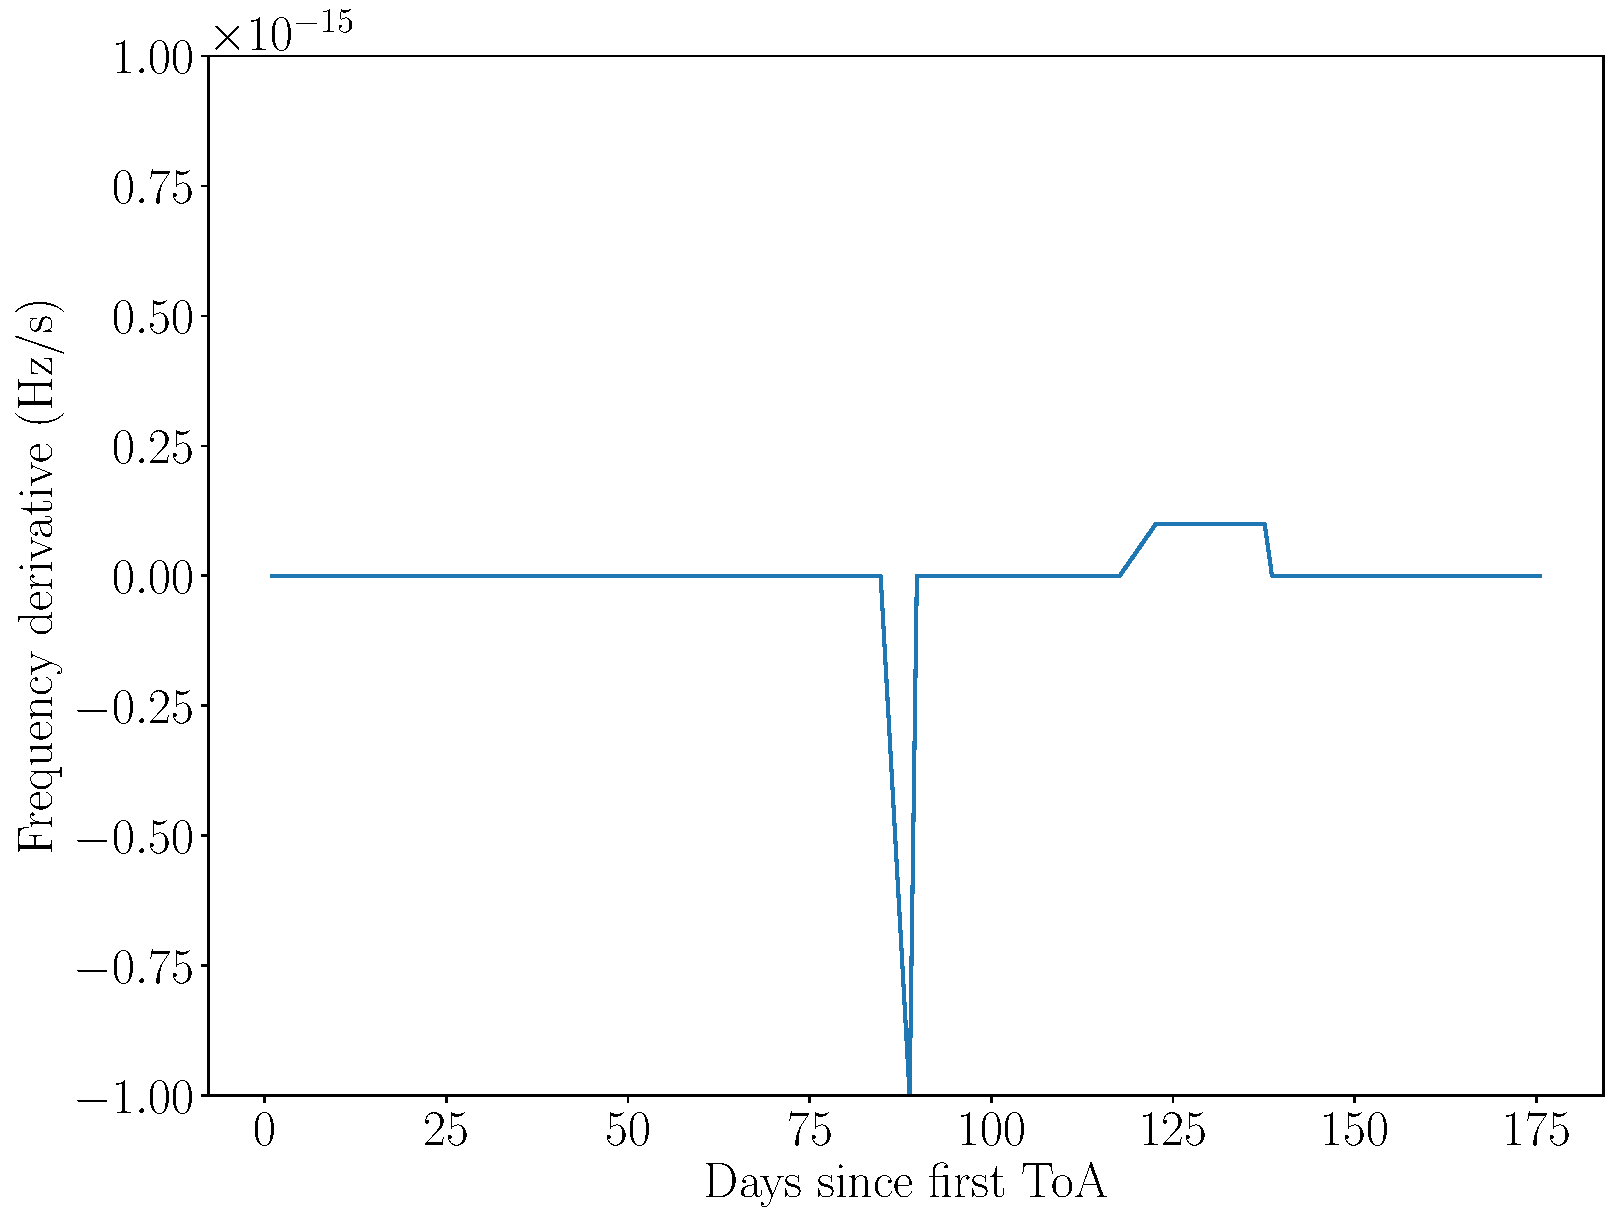
\includegraphics[width=0.49\textwidth]{figures/J1452-6036_fdot_path.pdf}
    \caption{Pointwise most likely paths $\hat{f}(t_n)$ \emph{(left)} and $\hat{\dot{f}}(t_n)$ \emph{(right)} from the demo PSR J1452$-$6036 analysis.}
    \label{fig:eg_paths}
\end{figure}

\subsubsection{\texttt{\{f, fdot\}\_posterior.pdf}}
These plots show heatmaps of the marginalised $f$ and $\dot{f}$ posterior probability densities, denoted $\gamma_f$ and $\gamma_{\dot{f}}$ respectively (see Section \ref{subsec:hidden_evo}).
We plot the heatmap of $\ln[\gamma_f]$ rather than $\gamma_f$ directly because $\gamma_f$ is frequently very strongly peaked, and heatmaps of $\gamma_f$ thus do not display well.
\begin{figure}
    \centering
    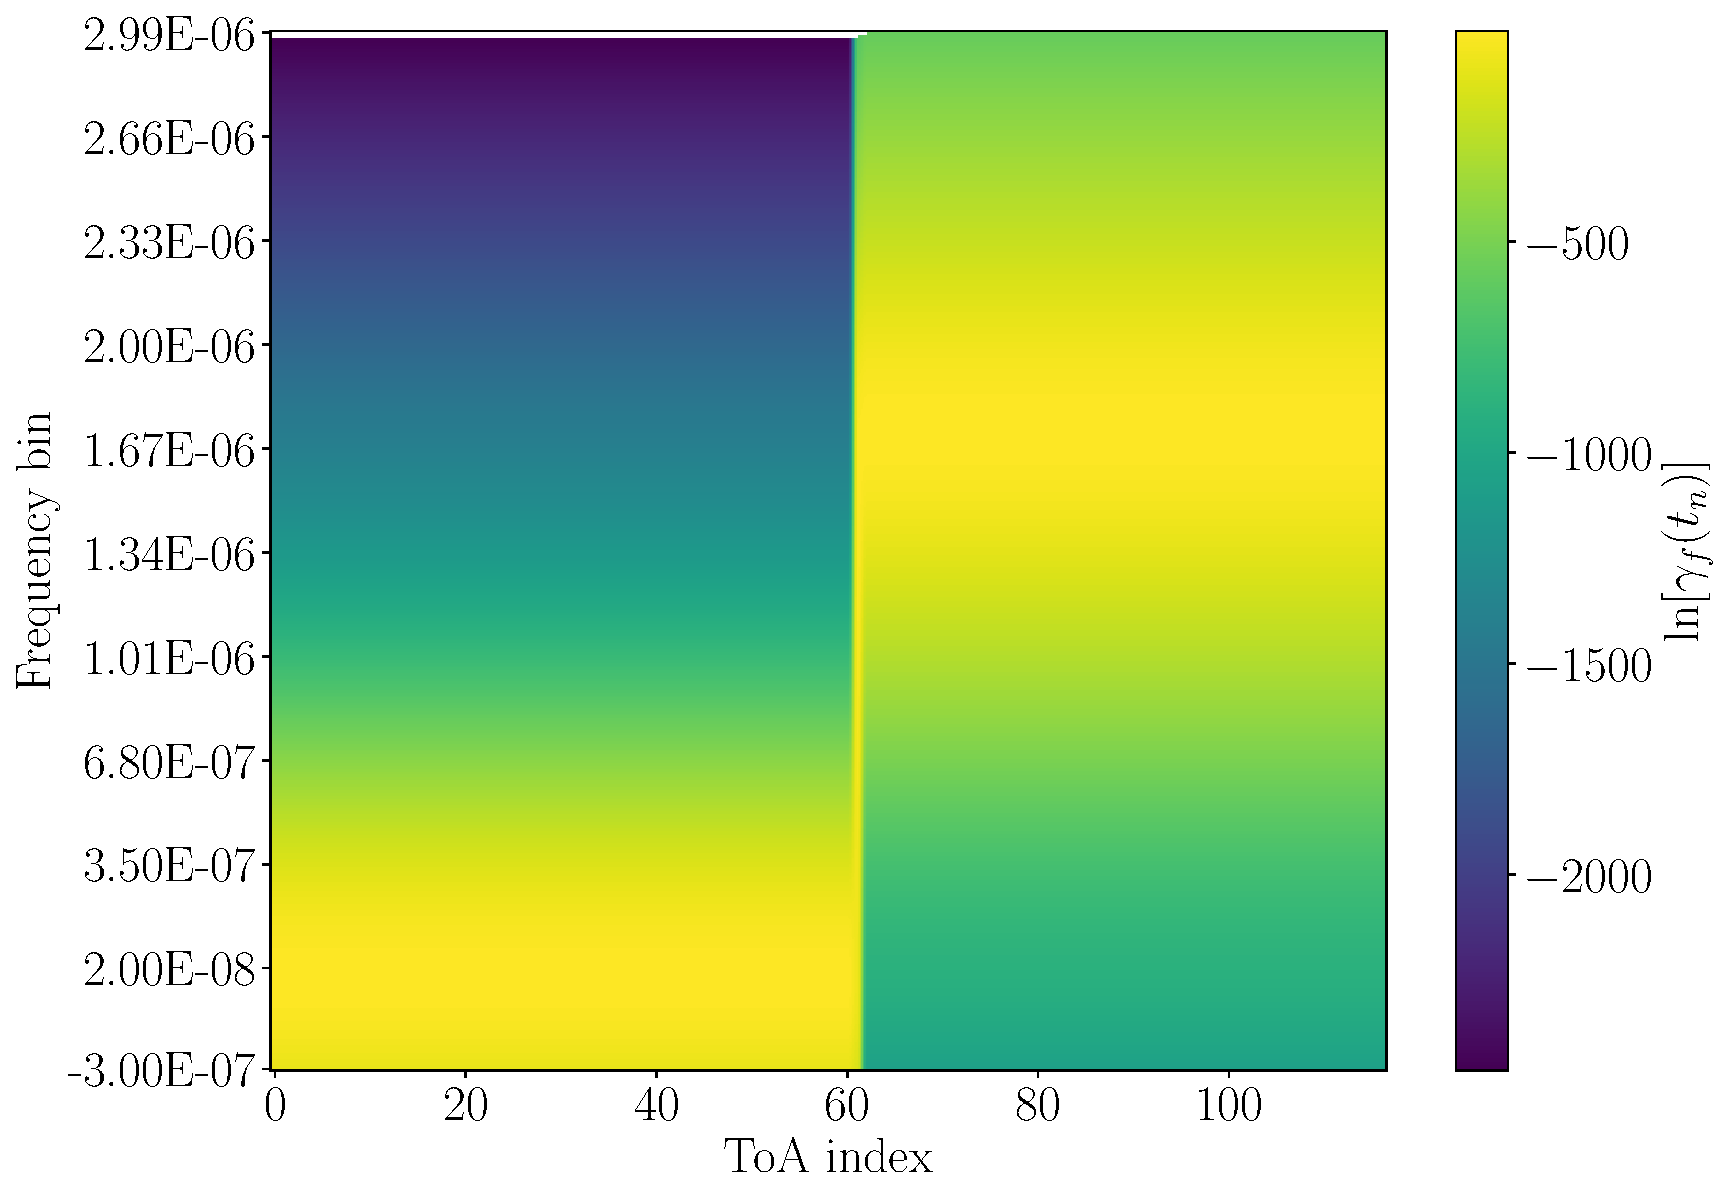
\includegraphics[width=0.49\textwidth]{figures/J1452-6036_f_posterior.pdf}
    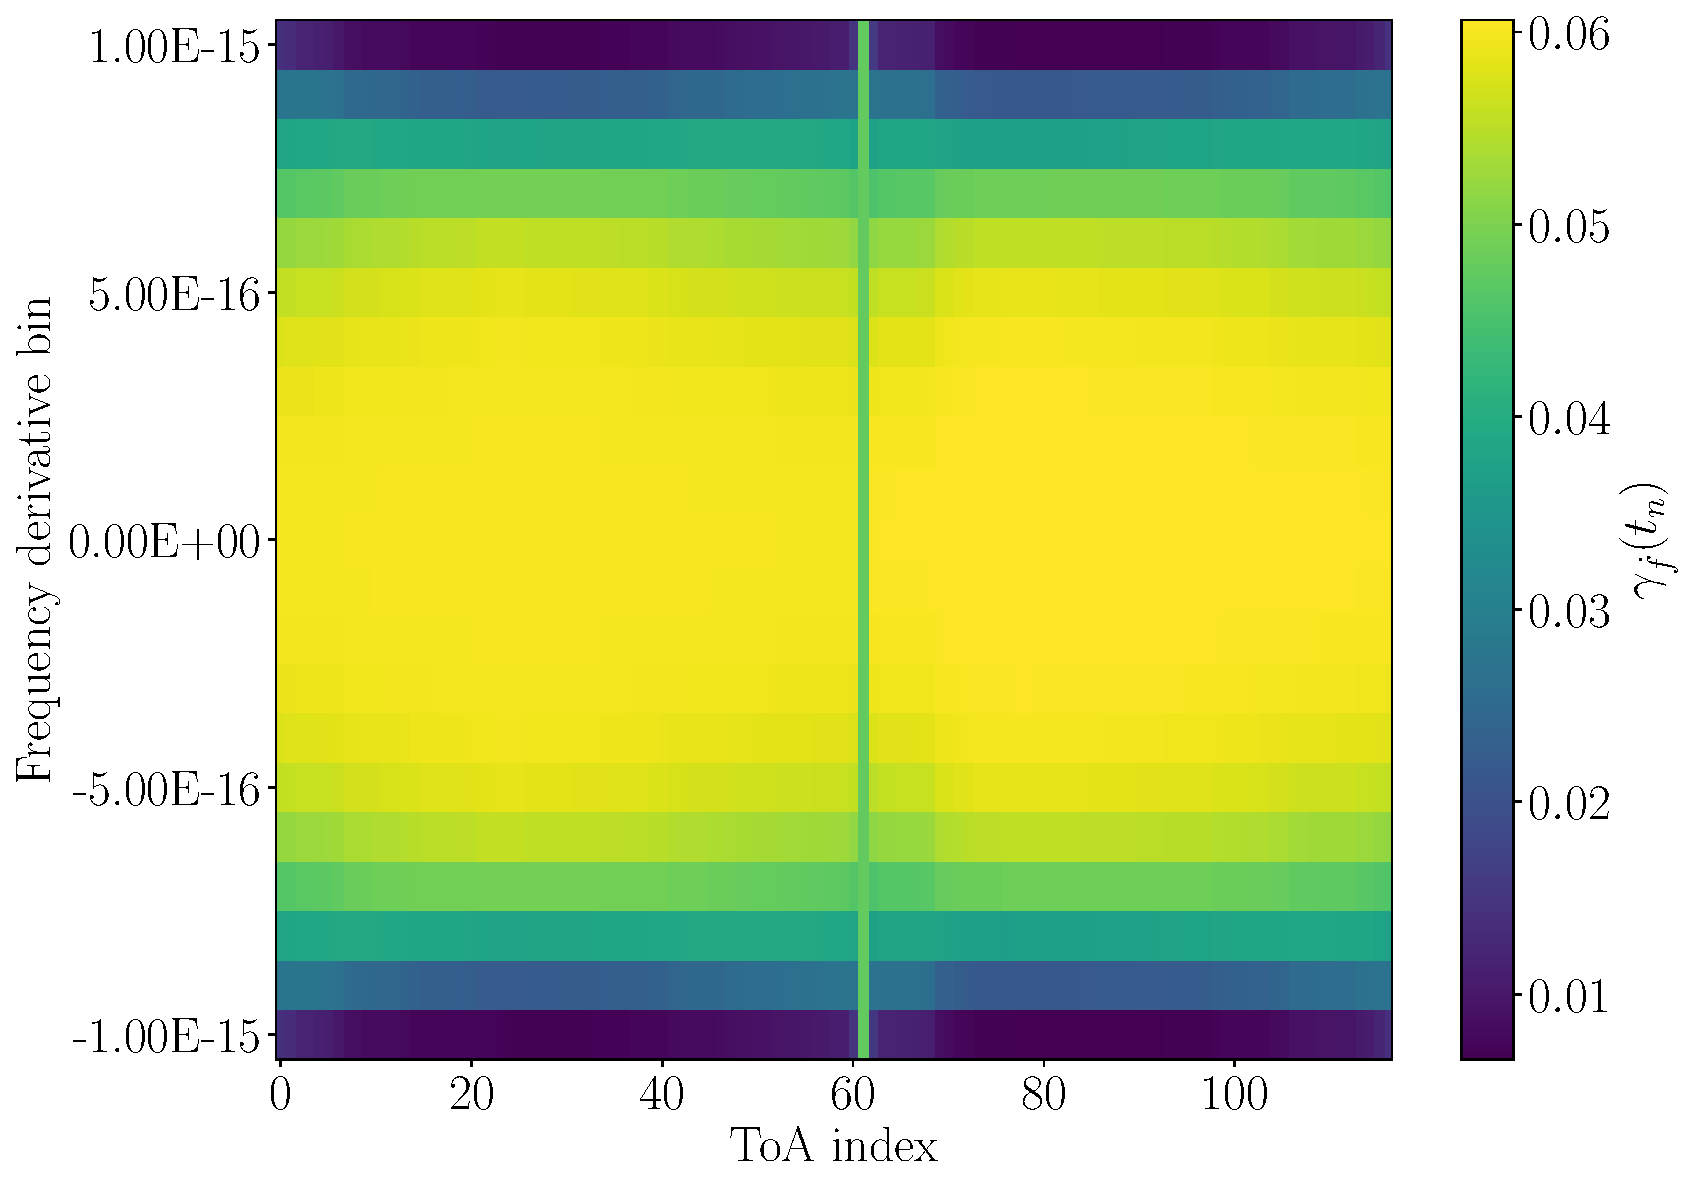
\includegraphics[width=0.49\textwidth]{figures/J1452-6036_fdot_posterior.pdf}
    \caption{Heatmaps of $\ln[\gamma_f(t_n)]$ \emph{(left)} and $\gamma_{\dot{f}}(t_n)$ \emph{(right)} from the demo PSR J1452$-$6036 analysis.}
    \label{fig:my_label}
\end{figure}
\bibliography{refs}{}
\end{document}